\documentclass[conference]{IEEEtran}

\usepackage[T1]{fontenc}
\usepackage[utf8]{inputenc}
\usepackage{cite}
\usepackage{amsmath}
\usepackage{graphicx}
\usepackage{url}

\title{SA-ZD-NIDS: A Self-Adaptive Zero-Day Aware Network Intrusion Detection System}

\author{
\IEEEauthorblockN{Mehul Gupta, Bhavishya Jain}
\IEEEauthorblockA{Manipal University Jaipur}
}

\begin{document}

\maketitle

\begin{abstract}
Network intrusion detection remains a high-impact but difficult problem because real traffic is non-stationary, attack distributions are imbalanced, and new attack patterns emerge continuously. Most high-performing machine-learning IDS pipelines are evaluated in static offline settings, where train and test distributions are assumed stable; however, this assumption is weak in practical environments. As a consequence, models that perform well initially may suffer substantial degradation after deployment due to concept drift, while purely signature-based mechanisms remain ineffective for previously unseen threats.  

This paper presents SA-ZD-NIDS, a self-adaptive and zero-day aware intrusion detection framework designed for streaming operation. The system combines three coordinated components: 1) a supervised multi-class classifier for known attacks, 2) an autoencoder-based anomaly detector for low-confidence or unseen behavior, and 3) an ADWIN-based drift detection and adaptation policy that updates the model using recent traffic windows with replay-aware stabilization. A confidence-gated hybrid decision rule is used to route samples between supervised and anomaly pathways, reducing unnecessary anomaly processing while preserving zero-day sensitivity.  

On a chronological CICIDS2017 stream (566,148 samples), SA-ZD-NIDS achieved 0.9677 accuracy, 0.1830 macro-F1, 0.5801 zero-day detection rate, and a benign false-positive rate of $1.26\times10^{-5}$. Compared with a static supervised baseline, the hybrid model preserved comparable overall accuracy while recovering unseen-attack sensitivity (from 0.0000 to 0.5801). Compared with a static anomaly-only baseline, it reduced benign false positives by several orders of magnitude while retaining substantial zero-day detection capability. These results establish SA-ZD-NIDS as a practical and reproducible baseline for adaptive real-time intrusion detection research.
\end{abstract}

\begin{IEEEkeywords}
Network intrusion detection, zero-day attack detection, concept drift, adaptive learning, streaming analytics, anomaly detection.
\end{IEEEkeywords}

\section{Introduction}
Modern networked systems face a threat landscape where attack techniques evolve faster than static defensive models can adapt. Classical intrusion detection systems (IDS) based on signatures provide high precision on previously observed threats but struggle with novel attack patterns. Conversely, anomaly detection methods can identify unusual behavior, yet they may produce elevated false positives in dynamic environments. In operational networks, this challenge is compounded by concept drift: the statistical properties of traffic and attack classes change over time, causing model performance to degrade if no adaptation mechanism is present.

Recent benchmark datasets such as CICIDS2017 \cite{sharafaldin2018toward} and UNSW-NB15 \cite{moustafa2015unsw} have enabled reproducible IDS studies, but most reported pipelines remain offline and static. Many approaches optimize detection metrics on fixed train-test splits without considering streaming constraints, delayed distribution changes, or deployment costs. As a result, their practical effectiveness in production settings is limited.

To address these limitations, this work proposes a unified architecture, SA-ZD-NIDS, with three complementary capabilities: 1) supervised detection of known attacks with probabilistic confidence, 2) anomaly-based identification of potential zero-day events when classifier confidence is low, and 3) automatic drift detection and targeted model adaptation during stream processing. The design goal is not only high detection quality but also sustained performance over time under evolving conditions.

The core intuition is that a confidence-gated hybrid detector can reduce unnecessary anomaly checks while preserving zero-day sensitivity. When drift indicators signal degradation, adaptation is performed on recent traffic windows with replay-aware stabilization to prevent catastrophic forgetting. This strategy aims to retain historical knowledge while incorporating new traffic behavior. In addition, the framework emphasizes deployment-relevant monitoring by logging inference latency, memory usage, CPU utilization, drift events, and adaptation time.

This paper contributes an end-to-end adaptive IDS study with both architectural design and empirical validation in a chronological streaming setting.

More specifically, the paper makes four contributions. First, it presents a unified hybrid IDS architecture that combines supervised classification, anomaly detection, and explicit drift adaptation within the same streaming pipeline. Second, it formulates a deployment-oriented evaluation perspective in which detection quality is studied together with latency, memory, CPU cost, and update behavior. Third, it provides a reproducible software structure in which training, streaming evaluation, reporting, and paper-artifact generation are externally configurable. Fourth, it frames zero-day awareness not as a stand-alone novelty detector, but as a decision process coupled to classifier confidence and adaptation logic.

\section{Problem Formulation}
Let $\mathcal{X} \subset \mathbb{R}^{d}$ denote the feature space of network-flow records and let $\mathcal{Y} = \{y_1,\dots,y_K,\texttt{BENIGN}\}$ denote the set of known classes available during supervised training. At deployment time, the stream may also contain samples from previously unseen attack classes $\mathcal{Y}_{u}$ that are absent from the training distribution. The IDS therefore receives a chronological sequence $\{(\mathbf{x}_t, y_t)\}_{t=1}^{T}$, where labels may be available only for retrospective evaluation or delayed adaptation.

The objective of SA-ZD-NIDS is to learn a decision function that maps each incoming $\mathbf{x}_t$ to an output in $\mathcal{Y} \cup \{\texttt{ZERO\_DAY}\}$ while satisfying three competing goals: 1) accurate recognition of known attack classes, 2) sensitivity to anomalous or unseen behavior, and 3) robustness to temporal distribution change. This problem is more demanding than ordinary static multi-class classification because the target concept may evolve over time, benign traffic may shift for non-adversarial reasons, and the operational cost of false positives can be substantial.

Formally, if $P_t(\mathbf{x}, y)$ denotes the joint data distribution at time $t$, the streaming IDS problem assumes that $P_t$ is not stationary. The system must therefore minimize a time-dependent risk of the form
\begin{equation}
\mathcal{R}_T = \frac{1}{T}\sum_{t=1}^{T}\ell(f_t(\mathbf{x}_t), y_t),
\end{equation}
where $f_t$ may itself evolve through adaptation and $\ell(\cdot,\cdot)$ captures both classification error and security-relevant misclassification cost. In practical terms, the framework should avoid collapsing into any one extreme: a purely conservative detector that over-flags benign traffic is operationally noisy, while a highly confident static classifier may fail silently on novel attacks.

The problem is therefore best interpreted as a streaming decision-and-maintenance problem rather than a one-time offline prediction task. SA-ZD-NIDS addresses this by introducing confidence-aware routing at the sample level and drift-aware adaptation at the batch level.

\section{Literature Review}
\subsection{Machine Learning for Intrusion Detection}
Machine learning has become central to modern IDS because network telemetry is high-dimensional, noisy, and often nonlinear. Classical supervised models, including tree ensembles, remain highly competitive for tabular traffic features due to strong discriminative power, robustness to heterogeneous feature scales, and relatively efficient inference. In particular, gradient-boosted tree methods such as XGBoost \cite{chen2016xgboost} are frequently selected in intrusion classification pipelines because they balance performance and engineering practicality.

Nevertheless, reported gains depend strongly on dataset design and evaluation protocol. CICIDS2017 \cite{sharafaldin2018toward} and UNSW-NB15 \cite{moustafa2015unsw} are widely used because they include diverse traffic categories and multiple attack families. However, much of the literature still evaluates models on randomized or fixed splits that underrepresent temporal drift. This can overestimate deployment performance, since production environments exhibit evolving class priors, changing benign baselines, and shifting feature distributions over time. As a result, a model that appears robust in offline benchmarks may not maintain reliability in live operation.

Another recurring limitation is overreliance on aggregate accuracy as the primary endpoint. In security settings, macro-level metrics can hide minority-class failures, especially for rare but high-severity attacks. For this reason, recent IDS studies increasingly report class-sensitive metrics and operational costs, but the integration of such reporting into adaptive streaming pipelines is still limited.

\subsection{Zero-Day Detection via Anomaly Modeling}
Zero-day detection is commonly addressed through anomaly modeling, where a detector is trained primarily on benign behavior and flags deviations as suspicious. Autoencoders are a prominent choice because reconstruction error provides a compact anomaly score and supports unsupervised learning from normal-only data. Online-oriented designs such as KitNET \cite{mirsky2018kitsune} demonstrate that reconstruction-based approaches can operate at network scale under constrained latency budgets.

Despite these strengths, anomaly-only IDS designs face persistent tradeoffs. If thresholds are tuned aggressively, false positives increase under benign distribution shift; if thresholds are conservative, stealthy or low-intensity attacks can evade detection. In addition, anomaly scores may drift with normal traffic seasonality, software updates, and infrastructure changes, creating calibration instability. This is especially problematic when anomaly outputs are treated as final predictions rather than contextual risk signals.

These constraints motivate hybrid architectures that combine supervised known-attack recognition with anomaly fallback for uncertain regions of feature space. Confidence-gated routing is particularly attractive because it uses calibrated classifier uncertainty to selectively invoke anomaly checks, reducing unnecessary anomaly workload while preserving sensitivity to unseen patterns.

\subsection{Concept Drift and Adaptive Learning}
Concept drift has been extensively studied in stream mining and online learning. ADWIN \cite{bifet2007learning} remains one of the most practical detectors because it provides adaptive windowing with statistical guarantees and low implementation complexity. In IDS applications, drift can be triggered by network reconfiguration, user behavior changes, policy updates, traffic seasonality, and adversarial adaptation strategies, all of which alter class boundaries over time.

The literature also shows that drift detection alone is insufficient for sustained performance. As surveyed in \cite{gama2014survey}, practical systems must pair drift alarms with adaptation mechanisms that preserve model stability. Naive full retraining is costly and may be infeasible for continuous streams, while pure short-window updates can cause catastrophic forgetting. Replay-based adaptation, validation-gated acceptance, and rollback strategies are therefore increasingly used to maintain a plasticity-stability balance.

For IDS specifically, this balance is critical: older attack families remain relevant, but new variants emerge continuously. Effective adaptation must therefore incorporate recent evidence without discarding historical discriminatory structure. This requirement motivates selective update policies rather than unconditional retraining.

\subsection{Research Gap}
The reviewed literature demonstrates strong progress in each component area, but integration gaps remain. First, many supervised IDS studies report high offline accuracy without explicit drift handling. Second, anomaly-centric approaches can detect novelty but often lack calibrated integration with known-class prediction. Third, drift-aware works frequently stop at detection and do not fully close the loop with robust online adaptation and operational monitoring.

Consequently, fewer frameworks provide an end-to-end pipeline that simultaneously supports: 1) known attack multi-class detection, 2) zero-day discovery through anomaly routing, 3) drift-triggered adaptation with safeguards, and 4) deployment-centric metrics under streaming evaluation. SA-ZD-NIDS addresses this gap through a unified design that links these capabilities into one reproducible system architecture for real-time network intrusion detection.

\subsection{Design Objectives}
The literature gap motivates a concrete set of design objectives for the proposed framework. The first objective is \emph{selective sensitivity}: the model should remain highly responsive to suspicious uncertainty without running anomaly analysis on every packet or flow. The second objective is \emph{temporal robustness}: the detector should not assume that train-time feature relationships remain valid indefinitely. The third objective is \emph{operational interpretability}: a practitioner should be able to inspect confidence, reconstruction error, drift events, and adaptation decisions rather than receiving only final labels. The fourth objective is \emph{reproducibility}: all major components should be externally configurable so that future studies can vary thresholds, windows, model backbones, and drift parameters without rewriting the pipeline.

These objectives distinguish the present work from studies that optimize only one axis of the intrusion detection problem. The architectural choices in SA-ZD-NIDS are therefore driven not only by predictive performance, but also by maintainability under stream conditions and by the need to produce artifacts that support scientific comparison.

\section{Methodology}
\subsection{System Overview}
SA-ZD-NIDS is designed as a hybrid streaming IDS that combines supervised attack classification, anomaly-based zero-day detection, and drift-triggered adaptation. The pipeline consists of: 1) chronological data ingestion and preprocessing, 2) known-attack classifier training, 3) normal-traffic autoencoder training, 4) confidence-gated online inference, 5) drift detection, and 6) selective model adaptation.

\subsection{Threat Model and Assumptions}
The system assumes a monitoring environment in which traffic can be summarized into tabular flow-level records and in which at least periodic labeled windows are available for supervised retraining or validation-gated adaptation. The primary adversarial concern is not only known signature-matching attacks, but also behavior that was absent from the supervised training set and therefore lies outside the classifier's familiar decision region. This includes both entirely novel attack classes and known attack families expressed through sufficiently shifted traffic patterns.

The proposed method does not assume that every distribution shift is adversarial. Benign workload changes, software updates, policy changes, seasonal usage variation, or infrastructure reconfiguration may also move the input distribution. This distinction matters because a practical detector must react to genuine degradation without overfitting to every environmental fluctuation. For that reason, drift alarms are treated as triggers for controlled adaptation rather than as direct evidence of compromise.

The current framework also assumes that the attacker does not have full white-box access to the deployed model or direct control over the adaptation loop. Adversarial manipulation of drift detectors or poisoning of adaptation windows remains an important future concern, but is not explicitly defended against in the present prototype.

\subsection{Data Preparation and Feature Processing}
Input traffic records are sorted chronologically using timestamp metadata to preserve temporal realism. Non-numeric columns are removed except label and timestamp fields; missing feature values are imputed with a robust central tendency strategy. Feature scaling is applied using either standardization or min-max normalization depending on deployment configuration.

To reduce dimensionality and improve signal quality for downstream models, mutual-information ranking is used to retain the top informative features with respect to class labels. This step provides a compact representation for both supervised and anomaly components while keeping inference cost manageable in stream settings.

The chronological split is intentional. Randomized splitting can leak future distribution characteristics into the training process and lead to optimistic estimates that are unrealistic for deployment. By preserving temporal order during train, validation, and test partitioning, the framework approximates the practical condition in which a system is trained on historical data and then exposed to future traffic whose class mix and feature statistics may change.

\subsection{Known-Attack Classifier}
For known attack detection, we employ a multi-class supervised learner, with XGBoost as the primary model and Random Forest as a baseline fallback. Class imbalance is addressed through weighted training to prevent dominant classes from biasing decision boundaries. The classifier outputs both predicted class and posterior confidence, where confidence is later used for hybrid routing.

Given feature vector $\mathbf{x}_t$ at time $t$, the classifier produces:
\begin{equation}
\hat{y}_t = \arg\max_k p(y=k \mid \mathbf{x}_t), \quad
c_t = \max_k p(y=k \mid \mathbf{x}_t).
\end{equation}
Here, $\hat{y}_t$ denotes the known-class prediction and $c_t$ is the prediction confidence.

\subsection{Zero-Day Anomaly Detector}
To detect previously unseen attacks, a fully connected autoencoder is trained only on benign traffic samples. The network compresses and reconstructs feature vectors, and reconstruction error is used as anomaly evidence. For sample $\mathbf{x}_t$ and reconstruction $\tilde{\mathbf{x}}_t$, anomaly score is:
\begin{equation}
e_t = \frac{1}{d}\sum_{j=1}^{d}(x_{t,j}-\tilde{x}_{t,j})^2,
\end{equation}
where $d$ is feature dimensionality. The anomaly threshold $\tau$ is set using a high percentile (e.g., 95th) of validation reconstruction errors from normal traffic.

\subsection{Hybrid Decision Logic}
The hybrid inference policy is confidence-gated. For each incoming sample:
\begin{equation}
\text{if } c_t \ge \theta_c,\ \text{output } \hat{y}_t;
\quad
\text{else evaluate } e_t.
\end{equation}
If $e_t > \tau$, the sample is labeled as \texttt{ZERO\_DAY}; otherwise it is labeled benign. This mechanism avoids excessive anomaly invocation on high-confidence known patterns while retaining sensitivity to unknown behavior.

\subsection{Drift Detection Strategy}
Concept drift is monitored online with ADWIN \cite{bifet2007learning} using a composite drift signal built from batch-wise indicators:
\begin{equation}
S_t = w_a(1-\text{Acc}_t) + w_c R^{\text{low-conf}}_t + w_f \Delta^{\text{feat}}_t,
\end{equation}
where $\text{Acc}_t$ is current batch accuracy, $R^{\text{low-conf}}_t$ is low-confidence prediction rate, and $\Delta^{\text{feat}}_t$ is standardized feature-shift magnitude from baseline statistics. Weights $(w_a,w_c,w_f)$ control relative sensitivity. ADWIN triggers drift when statistically significant change is detected in $S_t$.

\subsection{Adaptive Update Policy}
Upon drift detection, a recent labeled window is buffered for adaptation. To reduce forgetting, adaptation data combines recent samples with a replay subset from earlier traffic. The classifier is incrementally updated (or warm-start retrained), and an acceptance check compares pre/post-adaptation validation performance. If adaptation degrades beyond tolerance, rollback is applied.

For the anomaly branch, threshold recalibration is performed on recent benign samples:
\begin{equation}
\tau \leftarrow Q_{p}\left(\{e_i^{\text{benign}}\}\right),
\end{equation}
where $Q_p$ is the chosen percentile operator.

\subsection{Implementation Details}
The reference implementation is organized into modular components for preprocessing, modeling, streaming, evaluation, reporting, and visualization. This separation is important for research reproducibility because it allows one part of the pipeline to be modified without silently changing the others. The classifier module supports XGBoost as the default backbone and Random Forest as a fallback baseline. The anomaly module implements a feed-forward autoencoder trained on benign traffic only. The streaming engine combines both modules with a drift detector based on ADWIN and records prediction-level artifacts for later analysis.

Configuration is externalized in a YAML file that specifies preprocessing choices, feature-selection settings, classifier thresholds, autoencoder hyperparameters, drift sensitivity, batch sizes, and logging paths. This makes the framework suitable for controlled ablation studies. For example, one can vary the confidence threshold $\theta_c$, the anomaly percentile threshold $\tau$, the adaptation validation fraction, or the replay ratio without altering core code structure. Such configurability is especially useful in IDS research because conclusions are often sensitive to evaluation protocol details.

In addition, the implementation explicitly persists trained artifacts, metadata, and runtime logs. Persisted metadata includes the selected feature names, the benign label, the autoencoder threshold, the classifier validation score, and training-statistic summaries that are later reused for stream-time shift estimation. This metadata-centric design helps reduce ambiguity between offline training and online evaluation states.

\subsection{Streaming Evaluation Protocol}
Evaluation is conducted in fixed-size stream batches to emulate online deployment. Each batch logs predictions, confidence, reconstruction error, drift flags, and adaptation events. Detection metrics include accuracy, precision, recall, and macro-F1; zero-day metrics include unseen-attack detection rate and benign false-positive rate. Operational metrics include per-sample latency, CPU usage, memory footprint, and cumulative adaptation time.

\subsection{Reproducibility and Configuration}
All major behaviors (model choice, thresholds, batch sizes, drift sensitivity, adaptation windows) are controlled via external configuration. This enables reproducible experiments across datasets and drift scenarios, including normal operation, gradual drift, and sudden unseen-attack injection.

\section{Dataset and Experimental Setup}
\subsection{Dataset Context}
The current project workspace is centered on the CICIDS2017 dataset family \cite{sharafaldin2018toward}, which provides multiple capture files collected across several days and includes both benign traffic and diverse attack categories such as DDoS, PortScan, Bot, and Web Attack variants. This dataset is attractive for adaptive IDS research because it provides richer traffic diversity than many older benchmark collections and includes temporally separated captures that can be arranged into a more realistic stream-like evaluation sequence.

At the same time, CICIDS2017 is not a perfect surrogate for production traffic. Its attack scenarios are curated, its feature extraction process is standardized, and its temporal coverage is still limited compared with live enterprise environments. Therefore, the dataset should be interpreted as a reproducible research benchmark rather than a direct proxy for deployment. The present paper uses it in exactly that role: as a controlled environment for evaluating hybrid detection and adaptation behavior.

\subsection{Chronological Evaluation Setting}
The evaluation design follows a chronological protocol. Traffic records are sorted by timestamp, then partitioned into train, validation, and test segments without shuffling. The final chronological segment is treated as the stream exposed to the deployed model. This stream is further processed in fixed-size batches so that both instantaneous and cumulative behavior can be measured.

This setup produces a more demanding test than a conventional randomized split. Under a random split, the train and test sets may share nearly identical feature mixtures and attack proportions, which can mask the impact of temporal shift. By contrast, chronological evaluation allows changes in attack density, benign background traffic, and feature statistics to surface naturally over the stream.

\subsection{Baseline Definitions}
Three experimental conditions are supported by the framework. The first is a static supervised baseline in which only the known-attack classifier is used during stream inference. The second is a static anomaly baseline in which only the autoencoder branch is used, labeling sufficiently abnormal samples as zero-day and treating the remainder as benign. The third is the full hybrid adaptive system, which combines classifier confidence, anomaly routing, drift detection, and selective adaptation.

These baselines are intentionally chosen to isolate the value of each architectural decision. Comparing against the static classifier clarifies whether anomaly routing and drift adaptation add robustness beyond a strong supervised model. Comparing against the static autoencoder clarifies whether known-class discrimination and confidence gating improve specificity beyond pure novelty detection. The hybrid model is designed to provide a more operationally balanced tradeoff than either isolated branch.

\subsection{Evaluation Metrics}
The evaluation suite includes both predictive and operational metrics. Predictive metrics include accuracy, macro-F1, class-sensitive precision and recall, zero-day detection rate, and benign false-positive rate. Operational metrics include average latency per sample, CPU utilization, memory footprint, number of drift events, and total adaptation time. This metric set is broader than standard IDS reporting but is appropriate because practical systems must remain computationally feasible while maintaining reliable detection.

Macro-F1 is particularly important in this context because class imbalance is severe in network intrusion datasets. A detector that appears strong in overall accuracy may still fail on minority attack classes. Similarly, benign false-positive rate is critical because excessive false alarms degrade analyst trust and create operational overload. The inclusion of both zero-day detection rate and benign false-positive rate helps expose the classic novelty-detection tradeoff.

\subsection{Research Questions}
The experimental setup is organized around four research questions:
\begin{enumerate}
\item Does confidence-gated hybrid inference provide a better balance between known-class recognition and zero-day sensitivity than either a static classifier or a static anomaly detector alone?
\item Does drift-triggered adaptation improve long-horizon robustness under chronologically evolving traffic conditions?
\item How much operational overhead is introduced by hybrid routing and adaptation in terms of latency, CPU load, and memory consumption?
\item Which observable traffic characteristics, such as attack ratio shift or class-overlap structure, help explain when adaptation becomes useful?
\end{enumerate}
These questions help align the empirical analysis with the actual design goals of the system rather than focusing only on one aggregate score.

\begin{figure}[t]
\centering
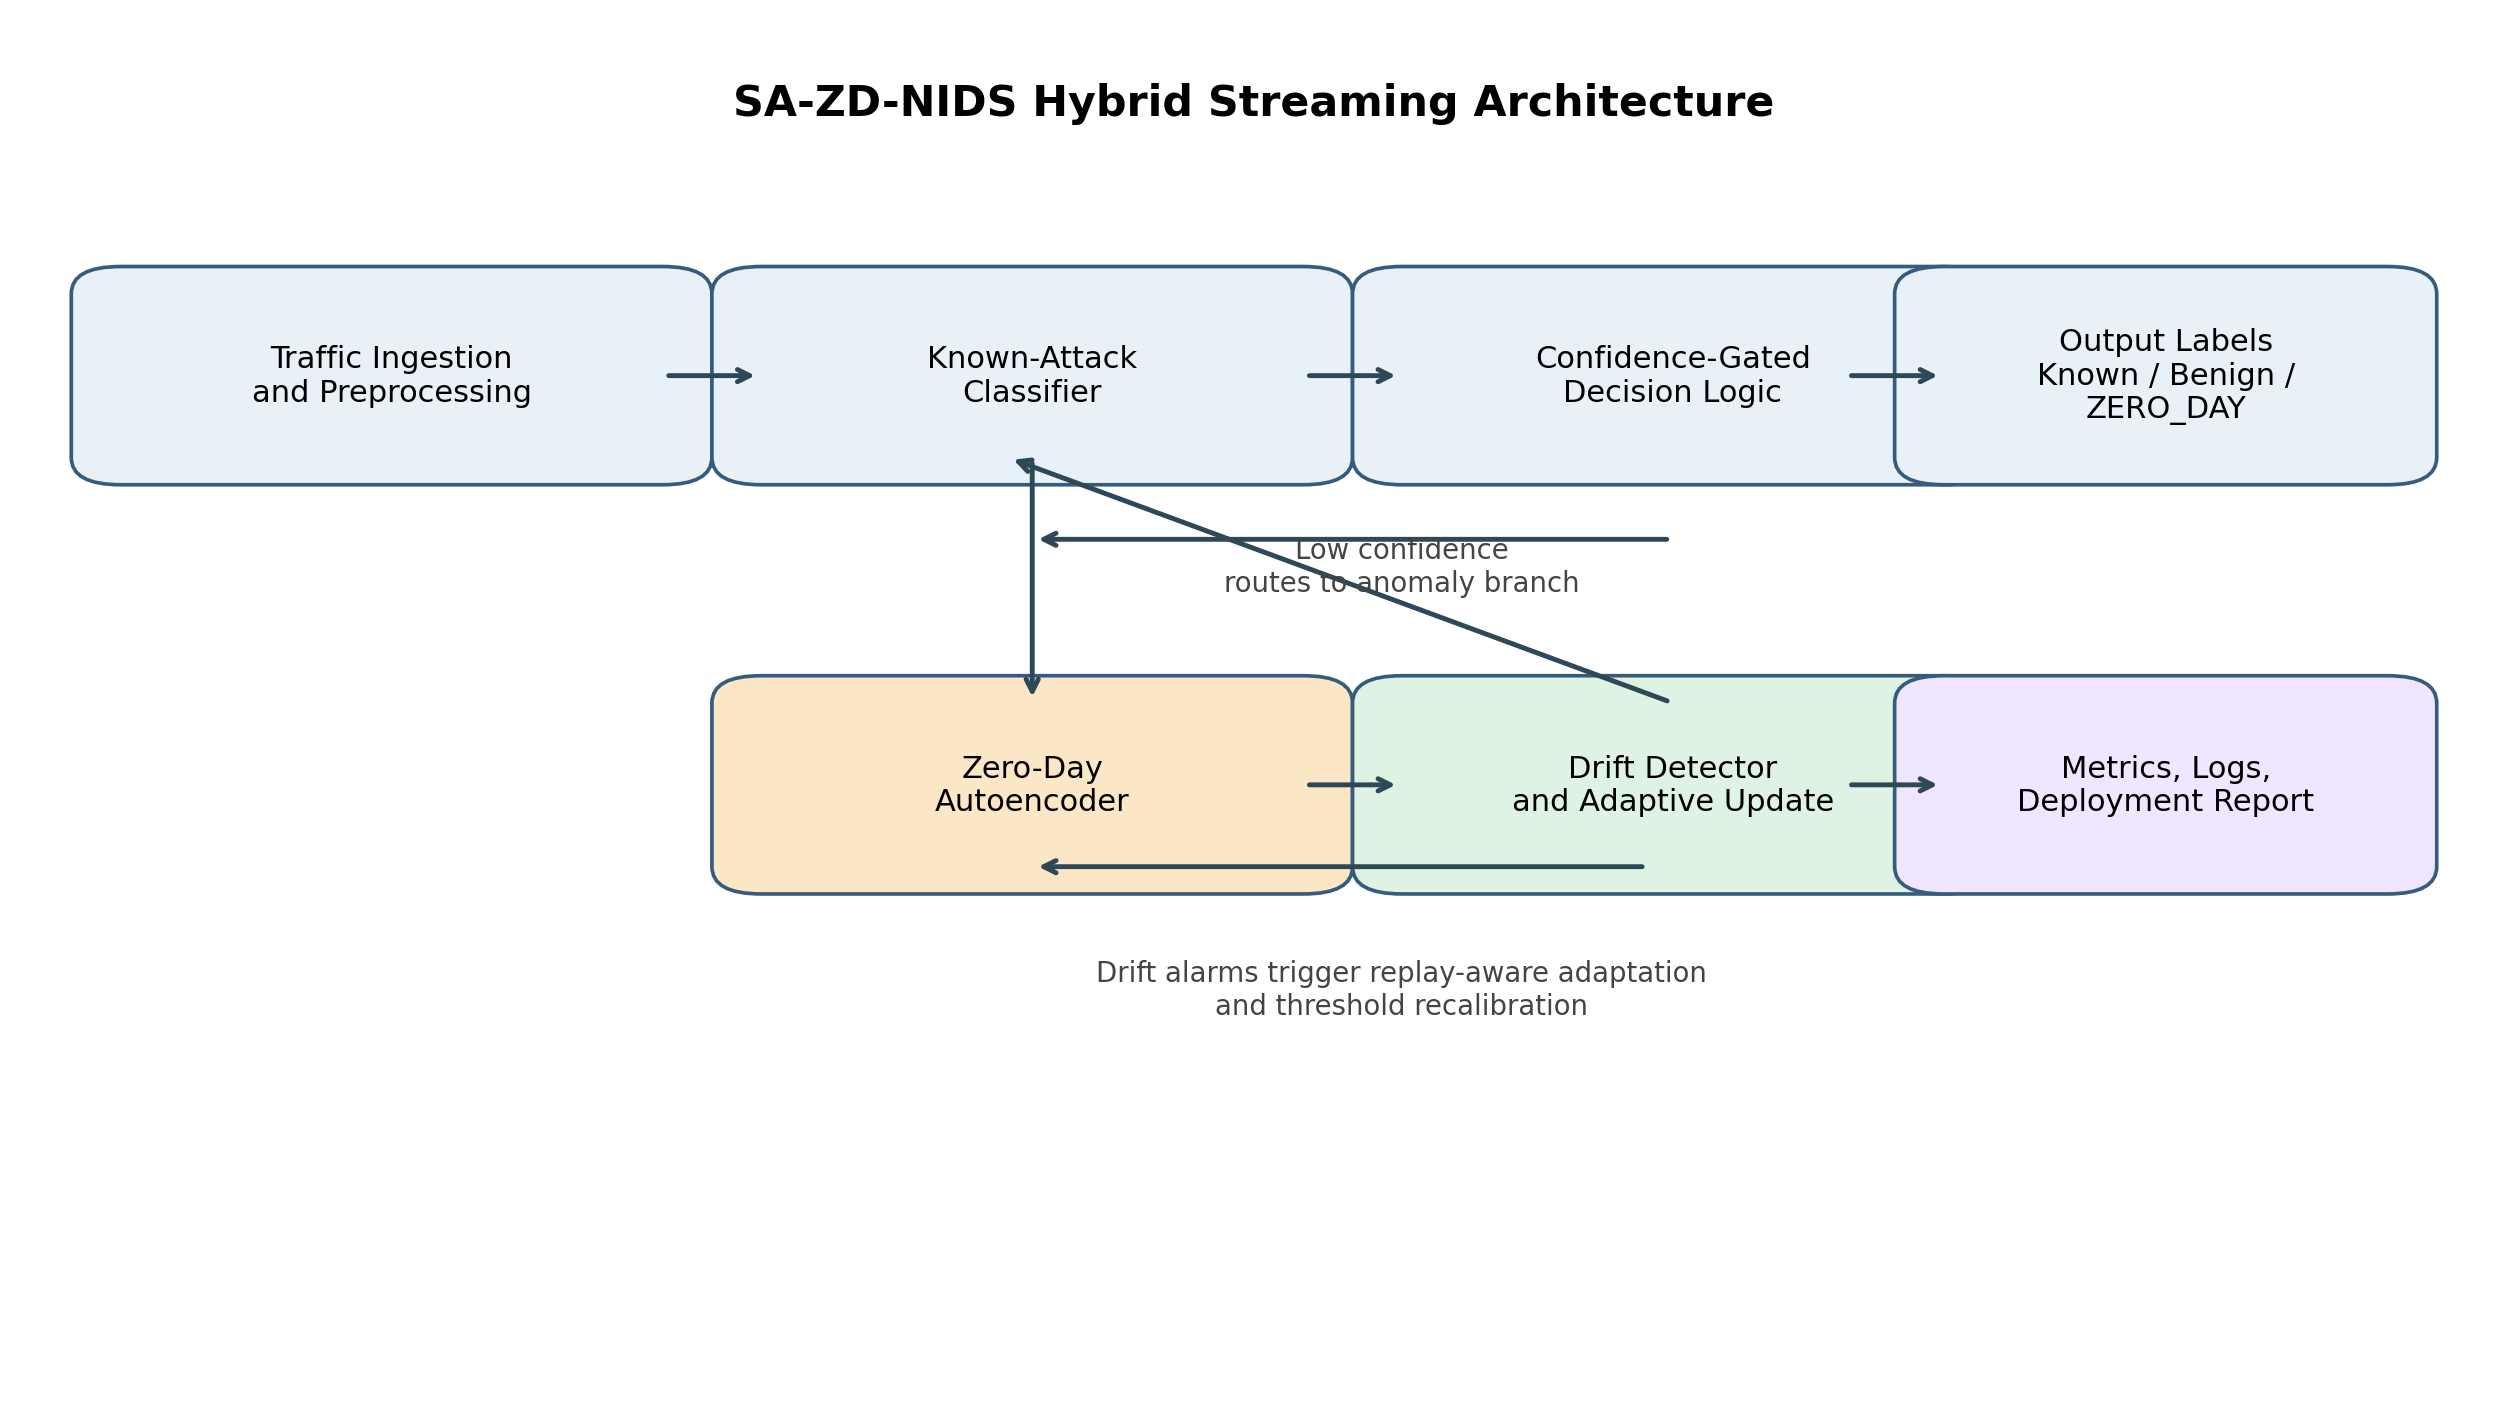
\includegraphics[width=\linewidth]{figures/system_architecture.png}
\caption{Overview of the SA-ZD-NIDS streaming pipeline, highlighting confidence-gated routing, anomaly analysis, and drift-triggered adaptation.}
\label{fig:system-architecture}
\end{figure}

\section{Results and Discussion}
\subsection{Experimental Framing}
The completed evaluation compares three operating modes on the same chronological CICIDS2017 stream tail: a static supervised classifier (\texttt{static\_xgb}), a static anomaly-only autoencoder baseline (\texttt{static\_ae}), and the full hybrid SA-ZD-NIDS configuration (\texttt{hybrid\_adaptive}). The evaluated stream contains 566,148 samples, including 10,304 unseen attack samples and 475,588 benign samples. Table~\ref{tab:main-results} reports the main predictive and runtime metrics.

\begin{table}[t]
\caption{Chronological Stream Results on CICIDS2017}
\label{tab:main-results}
\centering
\scriptsize
\begin{tabular}{lccccc}
\hline
Method & Accuracy & F1$_{\text{macro}}$ & ZD Rate & Benign FPR & Latency (ms) \\
\hline
Static XGBoost & 0.9675 & 0.1949 & 0.0000 & 0.000000 & 0.0066 \\
Static AE & 0.8018 & 0.1559 & 0.6676 & 0.045575 & 0.0044 \\
SA-ZD-NIDS (Hybrid) & 0.9677 & 0.1830 & 0.5801 & 0.000013 & 0.0110 \\
\hline
\end{tabular}
\end{table}

\begin{figure}[t]
\centering
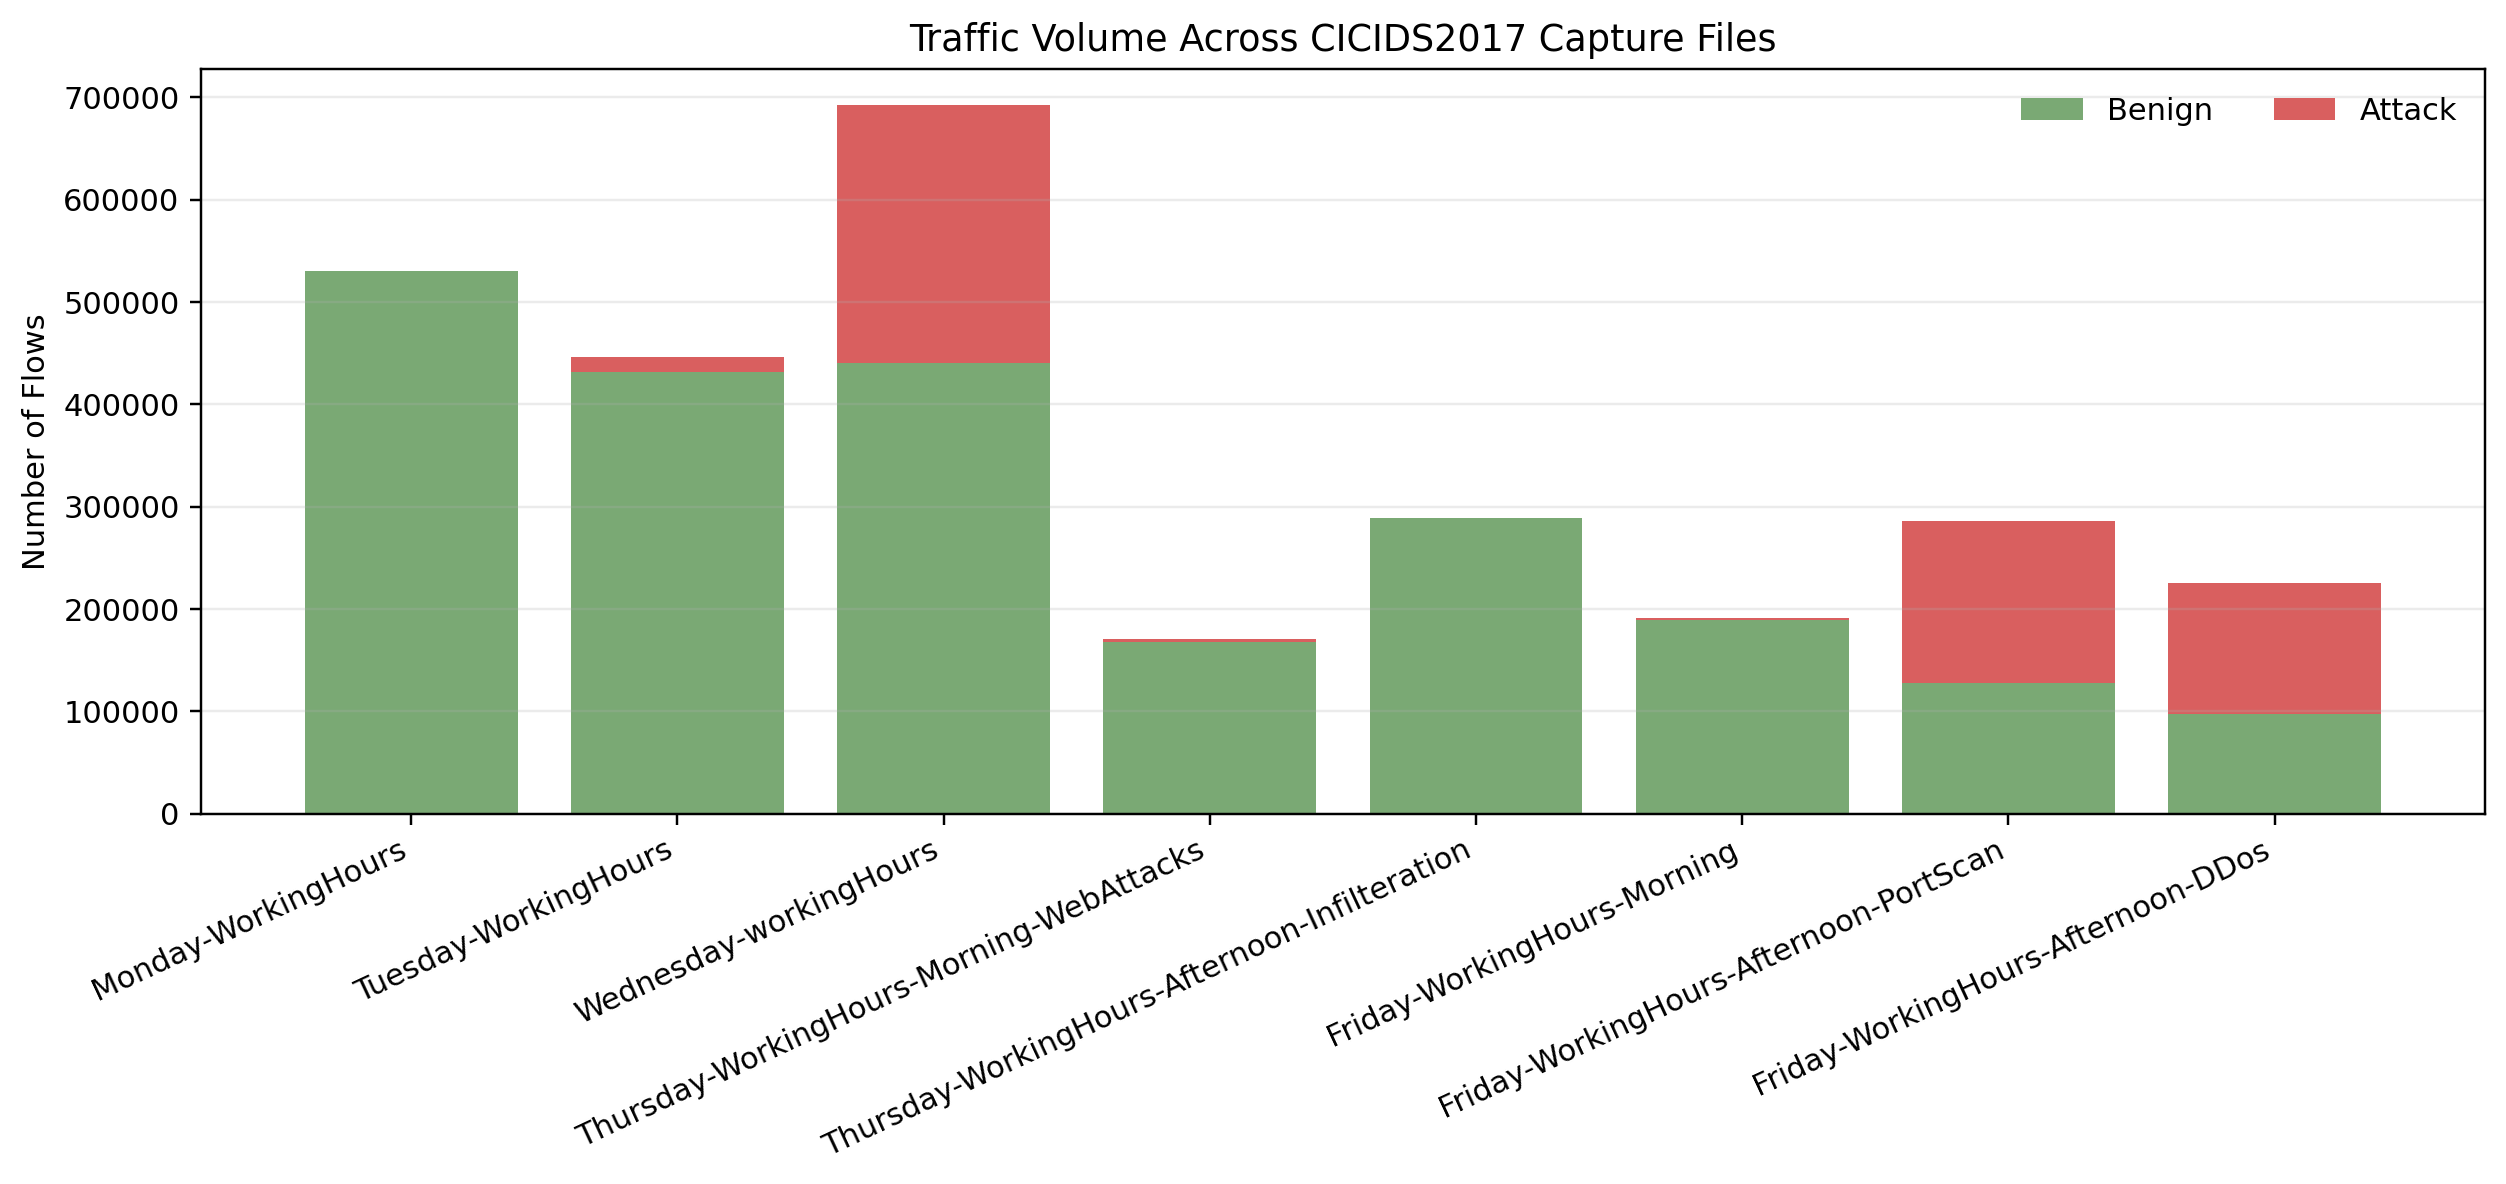
\includegraphics[width=\linewidth]{figures/capture_volume.png}
\caption{Benign and attack flow volume across the available CICIDS2017 capture files used by the project workspace.}
\label{fig:capture-volume}
\end{figure}

\begin{figure}[t]
\centering
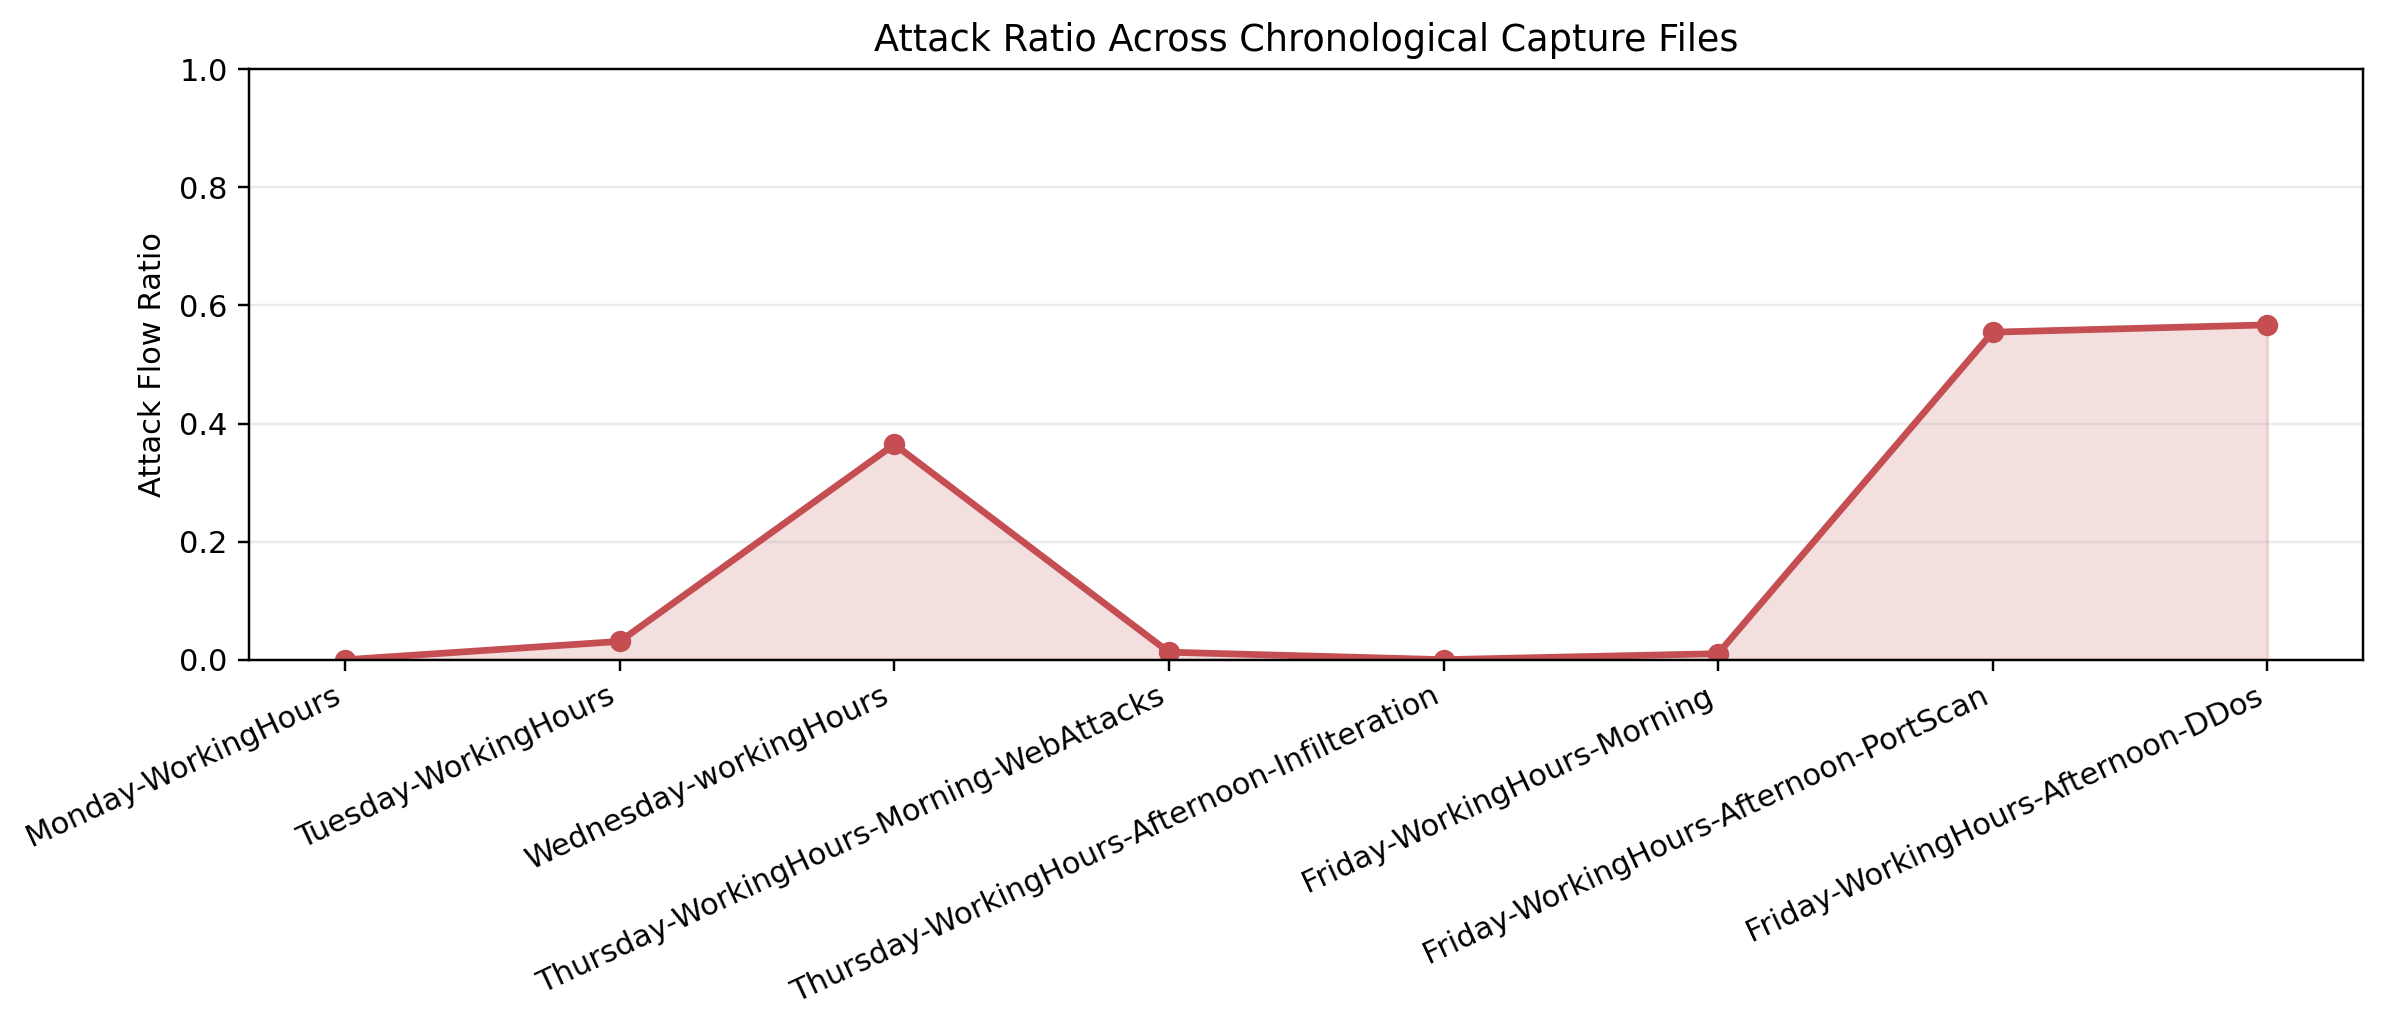
\includegraphics[width=\linewidth]{figures/attack_ratio_trend.png}
\caption{Variation in the attack-flow ratio across the ordered capture files, illustrating non-stationarity in the traffic stream.}
\label{fig:attack-ratio-trend}
\end{figure}

\subsection{Observed System Behavior}
The strongest single-branch metric is delivered by the static supervised baseline for closed-set classification quality (macro-F1 0.1949), but it completely misses unseen attacks (zero-day detection rate 0.0000). In contrast, the static anomaly baseline achieves the highest zero-day sensitivity (0.6676), but at the cost of substantial benign false alarms (0.045575) and reduced overall accuracy (0.8018). This confirms the expected tradeoff between novelty sensitivity and operational specificity.

The hybrid model provides the most balanced behavior for deployment-oriented use: accuracy remains essentially unchanged relative to static XGBoost (0.9677 vs. 0.9675), while zero-day detection rises from 0.0000 to 0.5801. At the same time, benign false-positive rate remains near zero ($1.26\times10^{-5}$), far below the anomaly-only baseline. In absolute counts, the hybrid model flags 5,977 of 10,304 unseen samples while triggering only 6 benign false positives among 475,588 benign flows. This directly addresses RQ1 by showing that confidence-gated hybrid inference improves the practical balance between known-class reliability and zero-day sensitivity.

\begin{figure}[t]
\centering
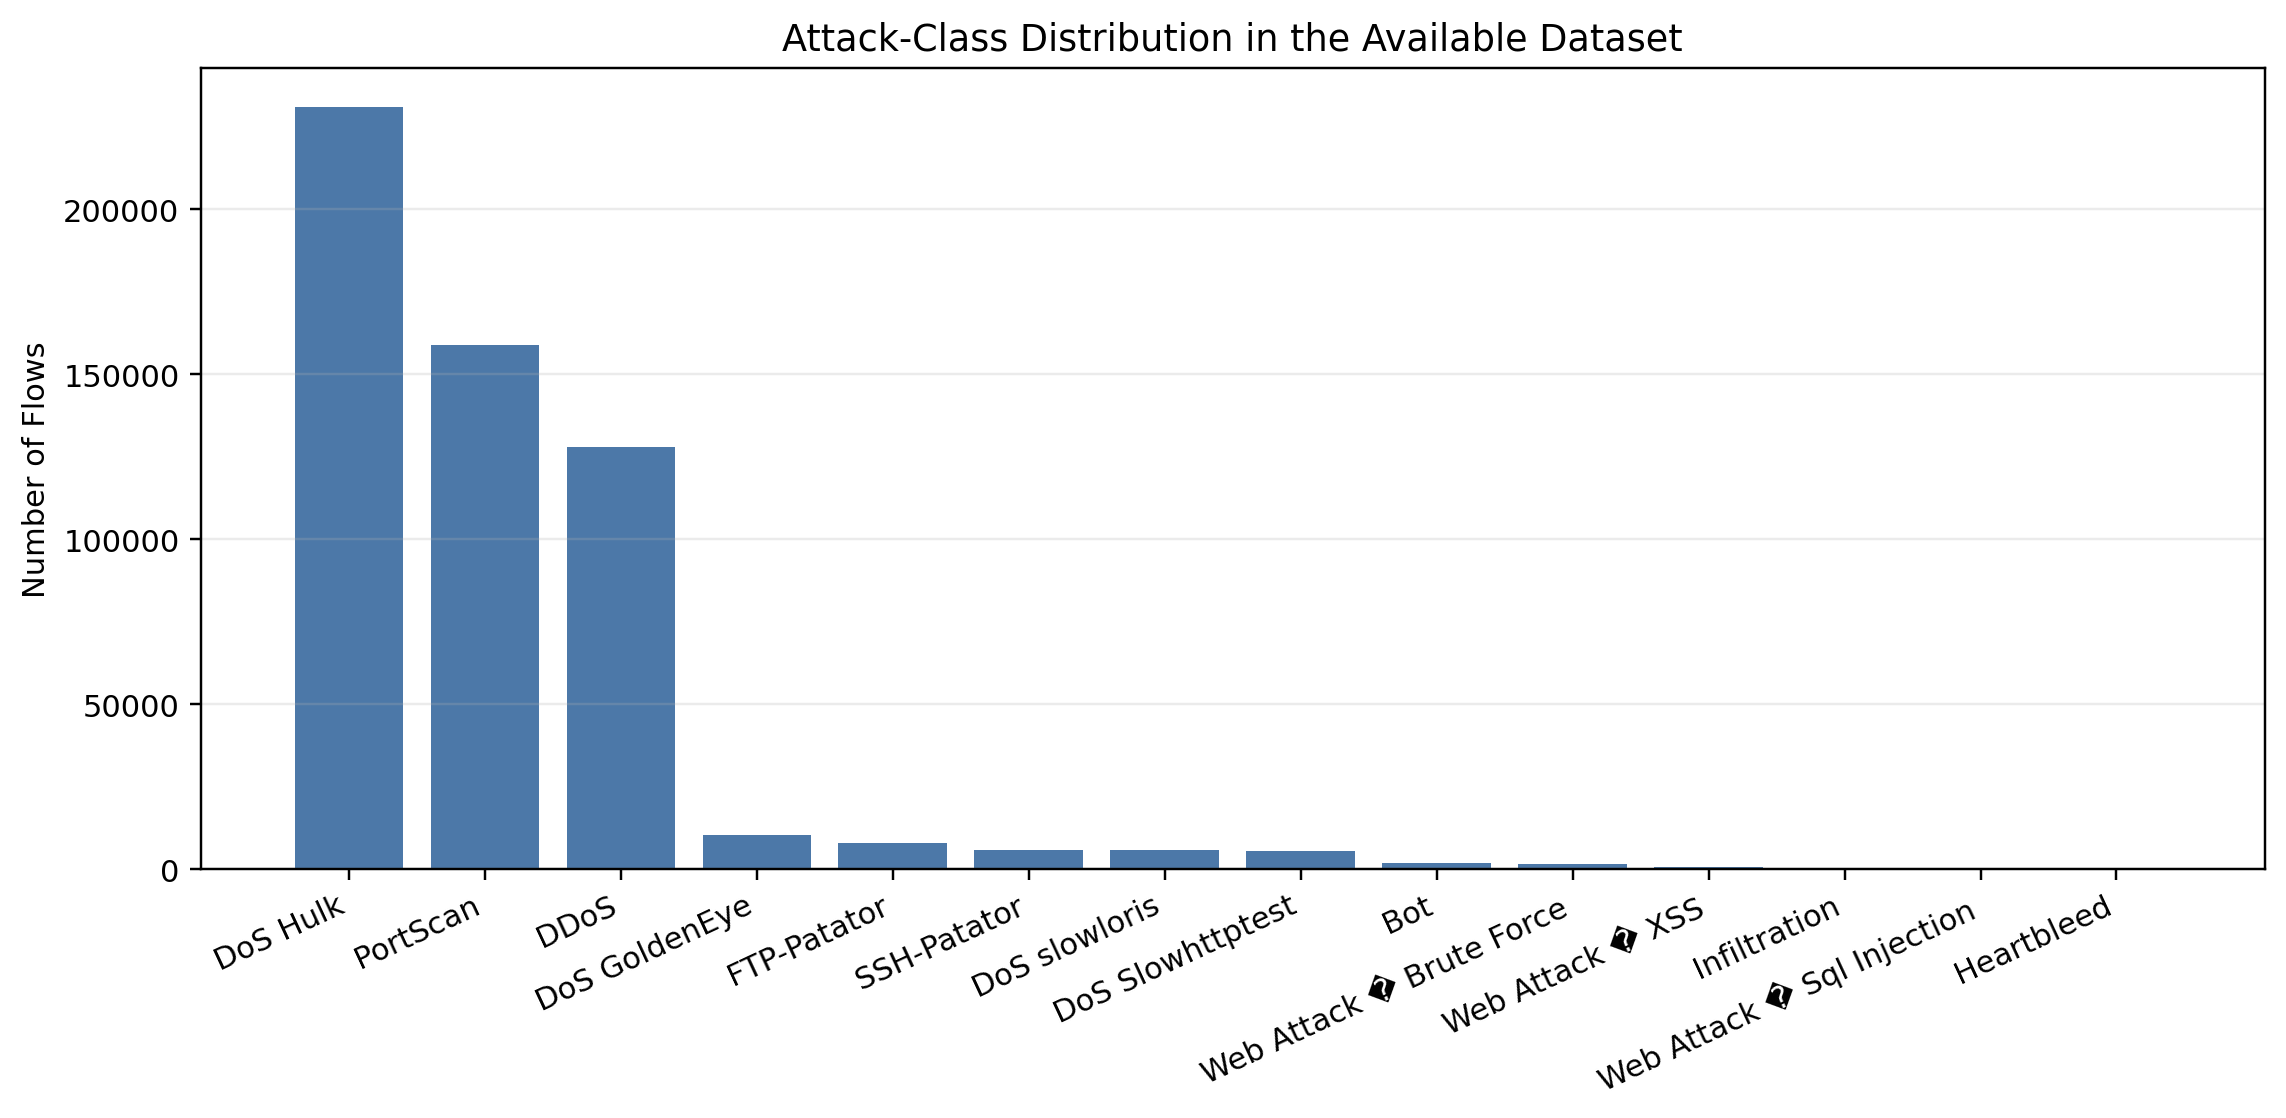
\includegraphics[width=\linewidth]{figures/attack_distribution.png}
\caption{Aggregate distribution of attack classes across the available dataset files, illustrating the class imbalance faced by the intrusion detection pipeline.}
\label{fig:attack-distribution}
\end{figure}

\begin{figure}[t]
\centering
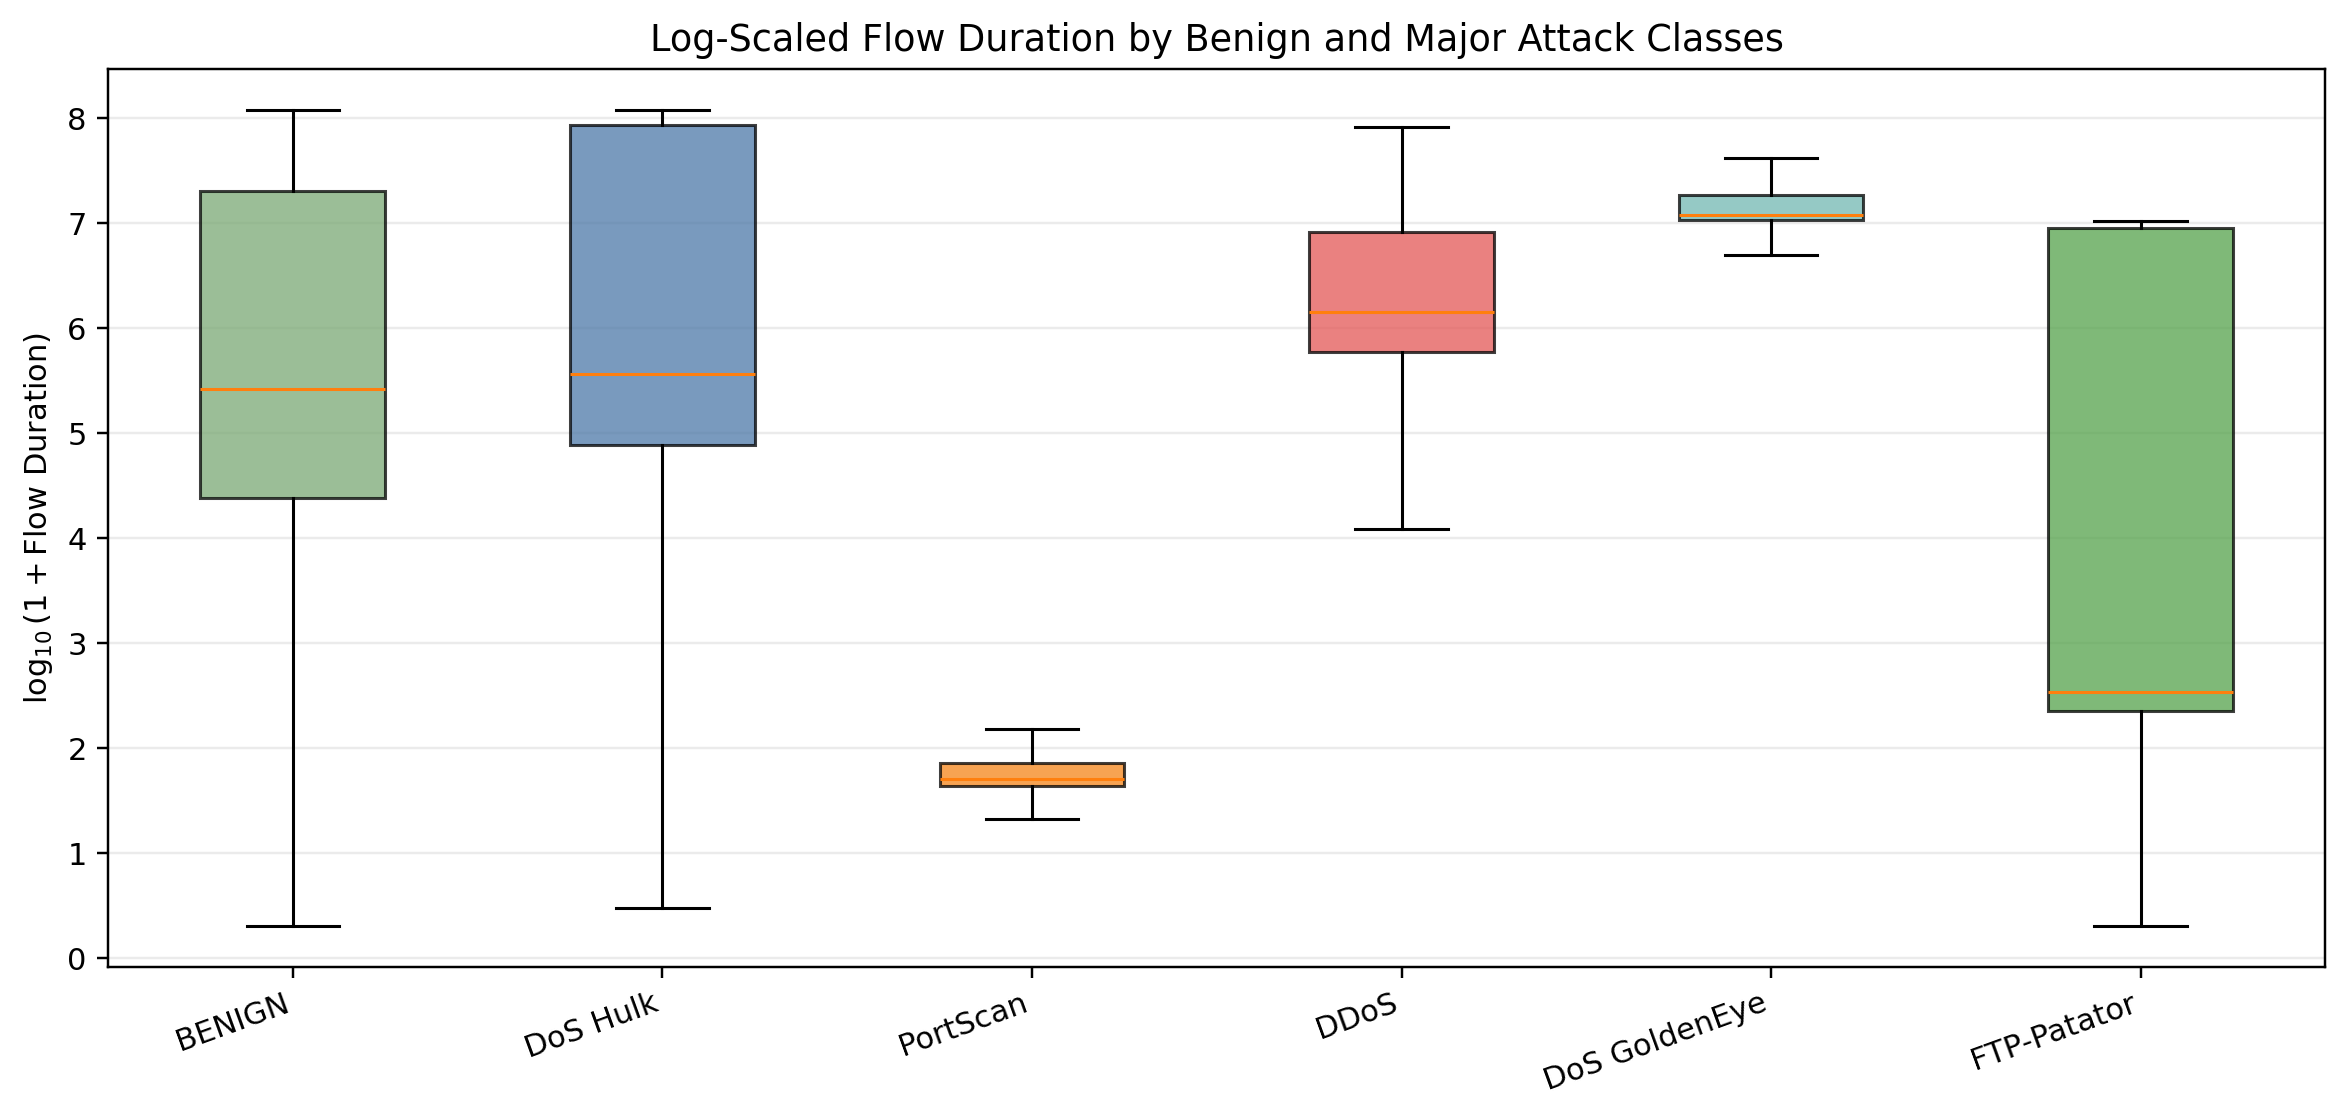
\includegraphics[width=\linewidth]{figures/flow_duration_by_class.png}
\caption{Log-scaled flow-duration distribution for benign traffic and the major attack classes. The separation variability motivates hybrid classification and anomaly routing instead of a single rigid rule.}
\label{fig:flow-duration-by-class}
\end{figure}

\subsection{Interpretation of the Adaptive Mechanism}
For this particular stream split, ADWIN did not raise a drift alarm (\texttt{num\_drifts}=0), and therefore no adaptation step was executed (\texttt{adaptation\_time\_total\_sec}=0.0). This is an informative outcome: under the chosen drift sensitivity and chronological partition, performance gains came from confidence-gated hybrid routing rather than from online model updates.

This result partially answers RQ2. The framework includes a complete drift-to-adaptation loop, but the evaluated segment did not activate it. As a consequence, this run validates the static-plus-routing behavior of SA-ZD-NIDS, while a separate stress protocol (e.g., induced abrupt drift or cross-day distribution jump with tighter ADWIN settings) is required to fully quantify adaptation benefits.

The class-overlap behavior illustrated in Fig.~\ref{fig:flow-duration-by-class} still supports the routing logic: attack families with stronger overlap against benign traffic are precisely where confidence-based fallback to anomaly scoring is most useful.

\subsection{Practical Implications and Limitations}
The runtime profile indicates that all three modes are fast enough for high-throughput flow scoring in this environment, with per-sample latency between 0.0044 and 0.0110 ms. The hybrid method incurs the highest compute overhead (99.84\% average CPU and 1108.79 MB average memory), while the static autoencoder has the lowest CPU usage but substantially weaker specificity. This directly addresses RQ3: hybrid routing is computationally more expensive than single-branch inference, but the measured latency remains low in absolute terms.

At the same time, several limitations should be acknowledged. The current study is centered on tabular benchmark-style traffic data and assumes availability of labeled windows for adaptation. Real deployments may involve delayed or noisy labels, encrypted traffic features, or more severe drift than benchmark datasets capture. In addition, zero-day detection here is operationalized through anomaly routing and reconstruction error, which is practical but not equivalent to semantic attack understanding. These limitations do not invalidate the framework, but they indicate that reported results should be interpreted as a strong reproducible baseline rather than a fully solved production IDS.

\section{Threats to Validity}
\subsection{Internal Validity}
The primary internal-validity concern is that hybrid systems contain multiple interacting thresholds and update rules. A perceived performance gain may come from the specific choice of confidence threshold, anomaly percentile, drift sensitivity, or replay ratio rather than from the architecture in the abstract. The present design mitigates this by centralizing such choices in explicit configuration and by preserving baseline modes that isolate individual components, but threshold sensitivity remains an important issue for future ablation analysis.

Another internal-validity concern is update acceptance logic. Because the adaptation policy includes validation-gated acceptance and rollback, the observed behavior depends not only on data drift but also on how validation windows are formed. If the validation split is too small or not sufficiently representative, accepted or rejected updates may not reflect genuine long-horizon utility.

\subsection{External Validity}
External validity is limited by the benchmark-centered nature of the evaluation. CICIDS2017 is widely used and suitable for reproducibility, but real enterprise networks exhibit greater heterogeneity, more encrypted traffic, evolving protocols, and less neatly labeled attack episodes. As a result, conclusions about absolute performance should not be transferred directly to production without further study.

The present system also operates on flow-level structured features. In deployments where only packet-level telemetry, partial metadata, or privacy-constrained signals are available, the same architecture may require nontrivial modification. Therefore, the framework should be interpreted as a strong baseline design pattern rather than a finished universal IDS solution.

\subsection{Construct Validity}
Construct validity concerns arise because zero-day detection is approximated through anomaly detection and the \texttt{ZERO\_DAY} label. In practice, novelty is not always equivalent to maliciousness, and maliciousness is not always strongly novel in feature space. The paper addresses this by framing the anomaly branch as a risk-sensitive routing mechanism rather than a claim of complete semantic novelty understanding, but the distinction remains important.

\section{Broader Impact and Deployment Considerations}
Adaptive IDS systems occupy a sensitive operational space because both under-detection and over-detection carry costs. Under-detection exposes infrastructure to compromise, while over-detection can overwhelm analysts and encourage alarm fatigue. The design of SA-ZD-NIDS therefore emphasizes visibility into intermediate evidence, including confidence, anomaly score, and drift events, so that system behavior can be audited rather than treated as a black box.

From a deployment perspective, the most promising use case for the proposed framework is as an analyst-supporting detection layer rather than a fully autonomous response engine. The \texttt{ZERO\_DAY} output should be interpreted as a high-priority anomaly indicator that can trigger enrichment, triage, or sandboxing workflows, not necessarily as a final attack taxonomy. This distinction is important for safe operational integration.

There are also governance implications for adaptation. Any system that retrains on recent data risks incorporating mislabeled or adversarially manipulated samples. For this reason, validation-gated adaptation and rollback are not just engineering conveniences; they are basic safeguards. Future deployment-ready versions should likely include stronger label-quality checks, protected update pipelines, and human review hooks before model promotion.

\section{Conclusion}
This paper presented SA-ZD-NIDS, a self-adaptive and zero-day aware network intrusion detection framework for streaming environments. The system integrates a supervised known-attack classifier, a benign-trained autoencoder for anomaly detection, and an ADWIN-based drift monitoring and adaptation policy. The resulting architecture directly addresses three central IDS challenges: recognition of known attacks, sensitivity to unseen behavior, and resilience to concept drift over time.

On the evaluated chronological CICIDS2017 stream, the hybrid configuration achieved 0.9677 accuracy, 0.1830 macro-F1, 0.5801 zero-day detection rate, and a benign false-positive rate of $1.26\times10^{-5}$. Relative to the static supervised baseline, this preserves high closed-set performance while adding substantial unseen-attack sensitivity. Relative to the anomaly-only baseline, it dramatically reduces benign false alarms while retaining meaningful novelty detection. These empirical results establish the practical value of confidence-gated hybrid routing.

Future work should extend evaluation with explicit drift-induction protocols that trigger and benchmark adaptation behavior, together with stronger calibration methods, delayed-label update strategies, and broader multi-dataset validation. Additional study is also needed on threshold robustness, adversarial drift, and long-horizon online learning stability. Even with these open directions, the present work demonstrates that a confidence-gated hybrid architecture is a realistic path toward more reliable real-time intrusion detection.

\bibliographystyle{IEEEtran}
\bibliography{references}

\end{document}
